\subsection{Load/Store Unit}

\begin{figure}[H]
	\centering
	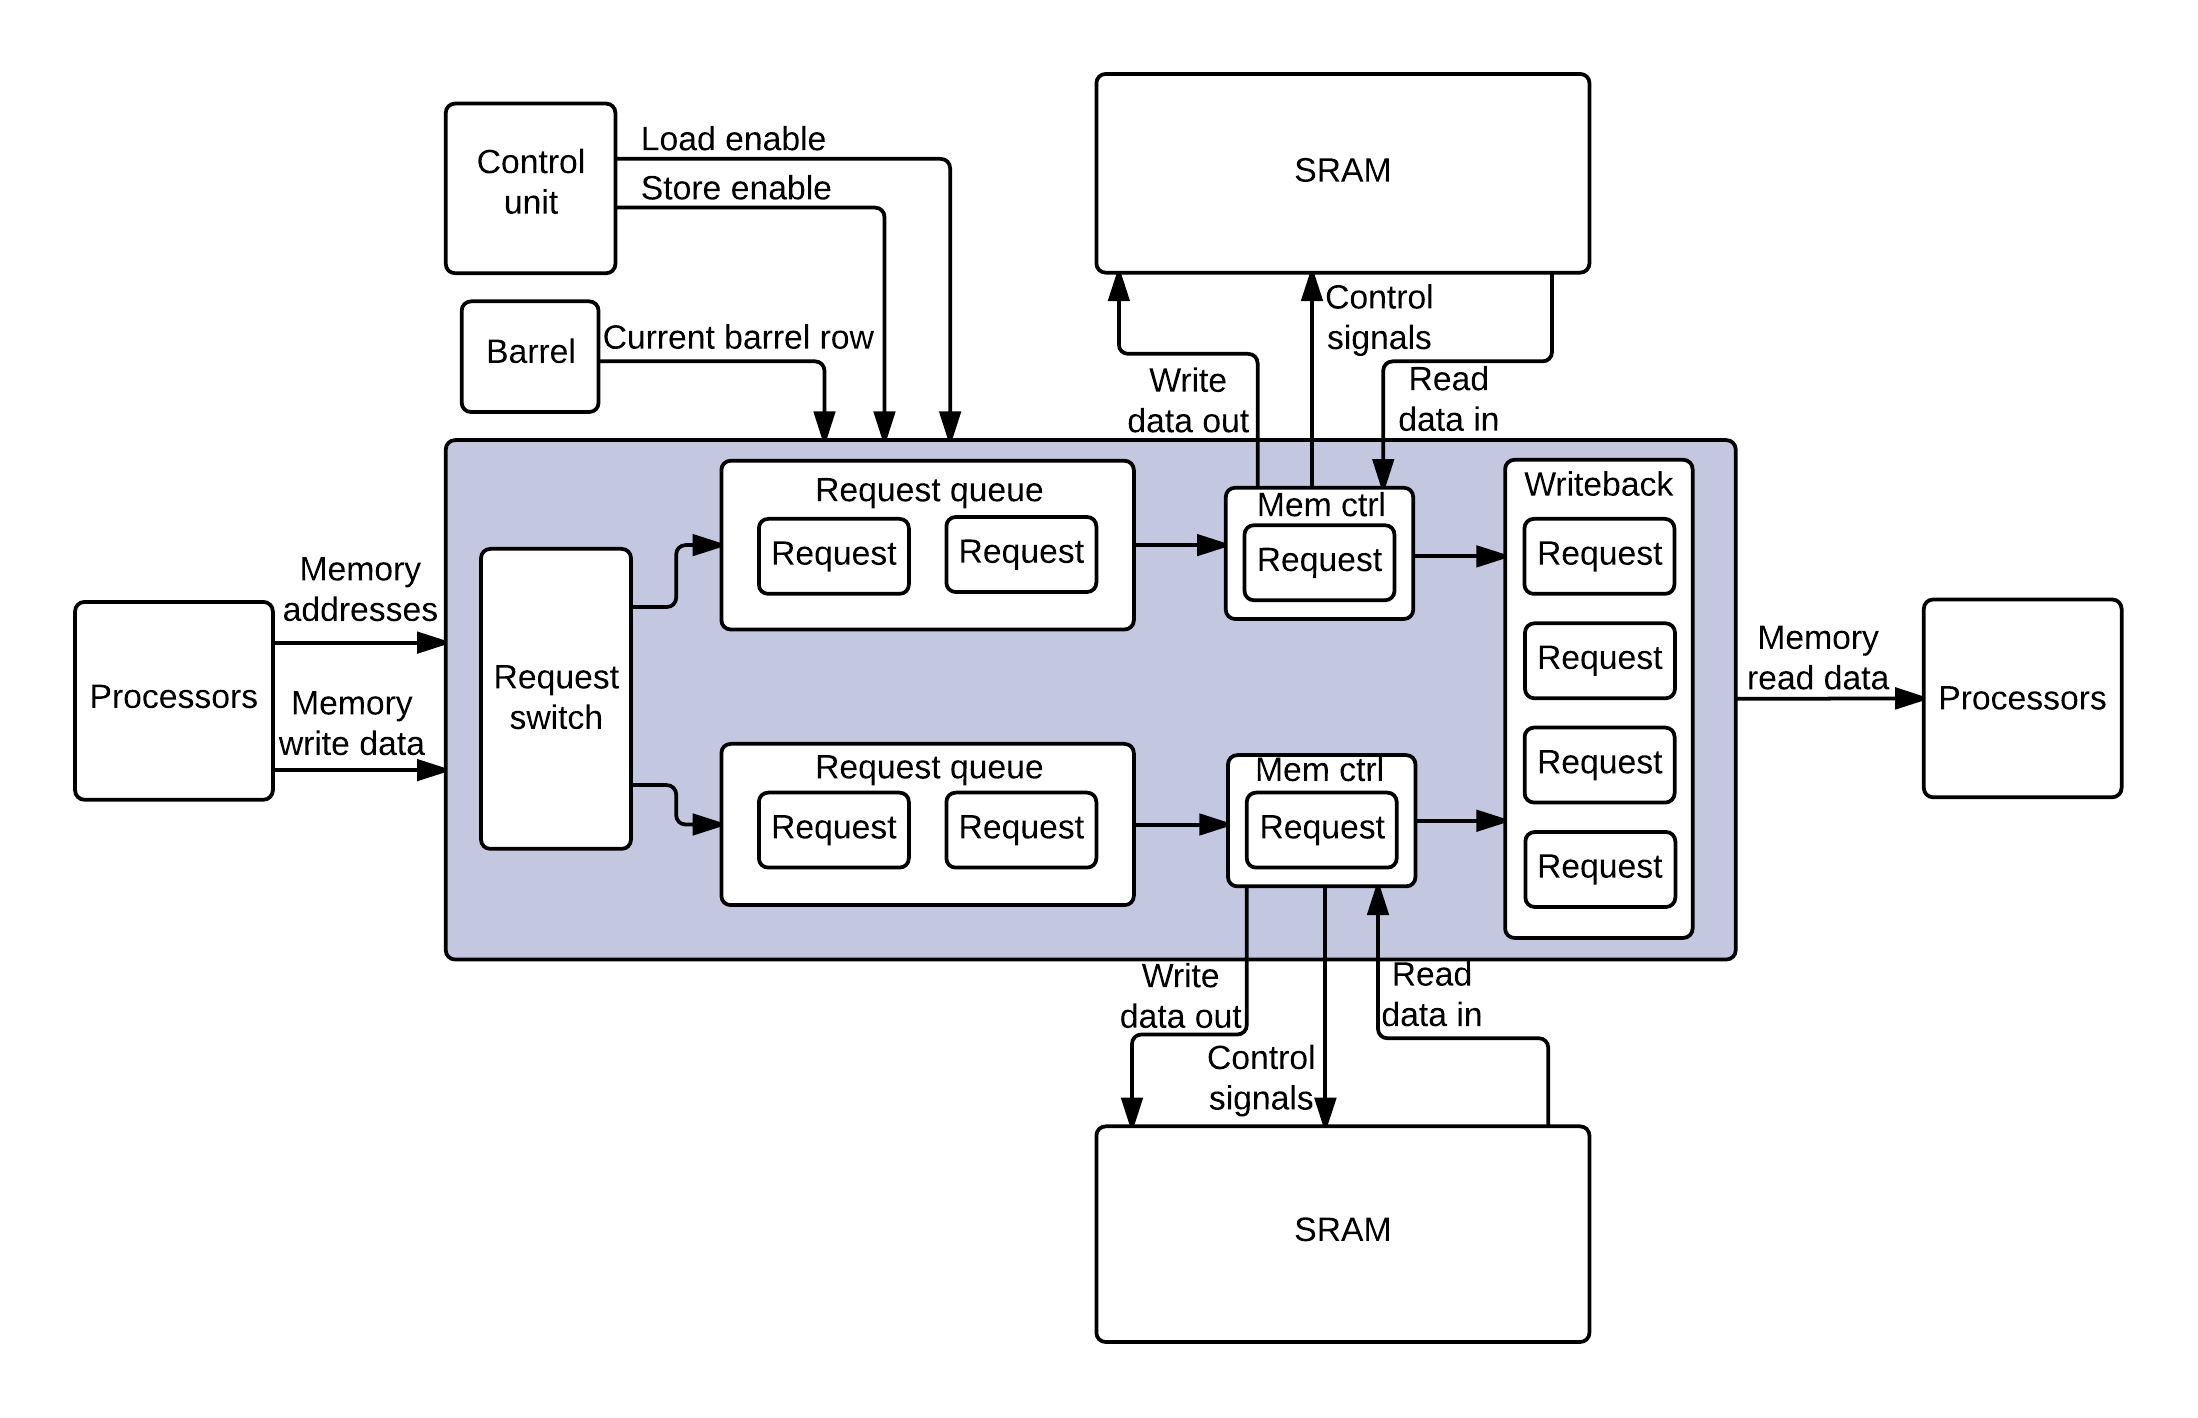
\includegraphics[width=\textwidth]{../gpu/diagrams/lsu.png}
	\caption{RTL of the load/store unit. Notice the dual queueing system to handle the interlaced SRAM.}
	\label{fig:lsu}
\end{figure}

A load/store unit, shown in figure \ref{fig:lsu}, is responsible for handling memory requests from the core processors.
The load/store unit of Demolicious needs to be capable of simultaneously servicing incoming requests from all the processor cores.
Requests are asynchronously carried out in the background, and replies are delivered directly into the appropriate registers of the threads that made the request.

Demolicious has two independent memory banks, each capable of reading or writing one word every cycle.
To maximize the throughput to the memory, a word-striping scheme is used:
The lowest bit of the memory address determines which bank holds that location.

Because there are two independent memory banks, the incoming requests are routed to two separate queues, one for each memory.
Each queue then feeds requests to its associated SRAM chip.
Read responses are then handed to the write-back unit, which delivers the data to the appropriate register file.

The queues are necessary because Demolicious has more processor cores than memory banks, so all the requests from a warp can not be completed in a single cycle, as discussed in section \ref{subsec:warps}.
The processor cores work in tandem, and issue requests simultaneously.
It takes several cycles to complete the requests for a single warp.
Since there is a limit to how many requests can be in the queue at any time, there is also a limit to how often requests can be issued.
